% Olympus v2 — RayNet environment -> agent connection (generic, abstract)
% raynet_agent_handoff.tex — companion strip to flow_agent_handoff.tex, same
% size and style: in RayNet there is no bridge and no exec. The environment
% simulates the flows and exposes them through a local RPC flow service
% (BaseManager on 127.0.0.1:<port> with a secret authkey); the agent is
% launched directly, connects with the addr + key it received, and drives
% the flow via set_cwnd / get_tcp_deepcc_info keyed by flow id.
% Sources: environments/raynet/env.py (_start_flow_service),
% common/flow_backend.py (_raynet_service, get_tcp_deepcc_info, set_cwnd).
% Compile standalone:  pdflatex raynet_agent_handoff.tex
\documentclass[tikz,border=2pt]{standalone}
\usepackage{tikz}
\usepackage{amssymb}
\usepackage{helvet}
\renewcommand{\familydefault}{\sfdefault}
\usetikzlibrary{arrows.meta,positioning,fit,backgrounds}

\begin{document}
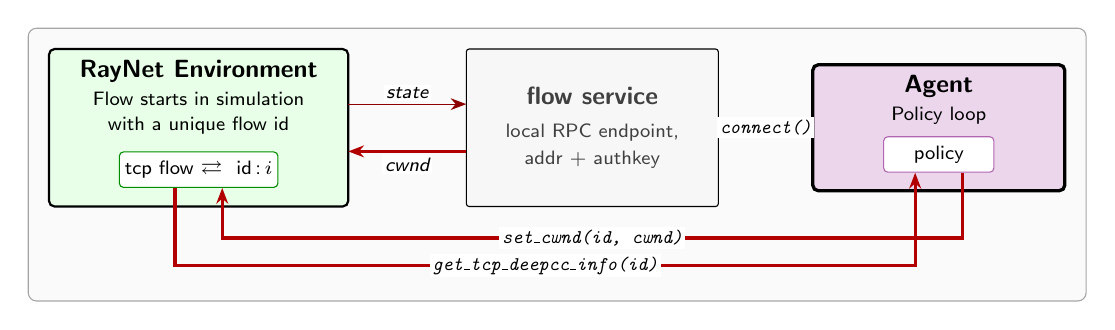
\begin{tikzpicture}[
  font=\small,
  >={Stealth[length=2mm]},
  proc/.style={draw,rounded corners=2pt,thick,minimum height=8mm,
               minimum width=24mm,align=center,fill=blue!7},
  net/.style={draw,rounded corners=2pt,thick,minimum height=8mm,
              minimum width=30mm,align=center,fill=green!9},
  agent/.style={proc,fill=violet!16,very thick},
  bridge/.style={draw,solid,thin,rounded corners=1pt,
                 minimum height=8mm,minimum width=24mm,align=center,
                 fill=black!3,text=black!75},
  flowbox/.style={draw,rounded corners=1.5pt,thin,draw=green!55!black,
                  fill=white,font=\scriptsize,inner sep=2pt,
                  minimum height=4.5mm},
  band/.style={draw,rounded corners=3pt,thin,draw=black!35,fill=black!2},
  subbox/.style={draw,rounded corners=1.5pt,thin,draw=violet!60,fill=white,
                 font=\scriptsize,inner sep=2pt,
                 minimum width=14mm,minimum height=4.5mm},
  data/.style={->,very thick,draw=red!70!black},
  tap/.style={->,thin,draw=red!55!black},
  cfg/.style={->,thick,draw=orange!80!black},
  lbl/.style={font=\scriptsize\itshape,fill=white,inner sep=1pt},
]

% ---- left: the environment, simulated flows keyed by flow id ----
\node[net,minimum width=38mm,minimum height=20mm] (env) at (0mm,0mm) {};
\node[align=center,anchor=north,inner sep=0pt] at ([yshift=-1.5mm]env.north)
     {\textbf{RayNet Environment}\\[-1pt]
      \scriptsize Flow starts in simulation\\[-2pt]
      \scriptsize with a unique flow id};
\node[flowbox,anchor=south] at ([yshift=2.5mm]env.south) (tcpflow)
     {tcp flow $\rightleftarrows$\ \ id\,:\,$i$};

% ---- middle: the RPC flow service the environment exposes ----
\node[bridge,minimum width=32mm,minimum height=20mm] (service) at (50mm,0mm)
     {\textbf{flow service}\\[1pt]
      \scriptsize local RPC endpoint,\\[-1pt]
      \scriptsize addr $+$ authkey};

% ---- right: the agent, launched directly (no bridge, no exec) ----
\node[agent,minimum width=32mm,minimum height=16mm] (agentbox) at (94mm,0mm) {};
\node[align=center,anchor=north,inner sep=0pt] at ([yshift=-1.5mm]agentbox.north)
     {\textbf{Agent}\\[-1pt]
      \scriptsize Policy loop};
\node[subbox,anchor=south] at ([yshift=2.5mm]agentbox.south) (policy)
     {policy};

% backdrop card around the whole connection
\begin{scope}[on background layer]
  \coordinate (loopbot) at (45mm,-19.5mm);
  \node[band,fit=(env)(service)(agentbox)(loopbot),inner sep=2.5mm]
       (backdrop) {};
\end{scope}

% the environment feeds the service flow state; actions flow back into it
\draw[tap]  (19mm,3mm)  -- node[lbl,above=0.3mm]{state}  (34mm,3mm);
\draw[data] (34mm,-3mm) -- node[lbl,below=0.3mm]{cwnd}   (19mm,-3mm);

% the agent connects with the addr + key it was given
\draw[cfg,very thick] (78mm,0mm)
      -- node[lbl]{\texttt{connect()}} (66mm,0mm);

% control loop over the RPC service: policy <-> flow, keyed by flow id,
% routed under the strip with nested orthogonal lines
\coordinate (setline) at (0mm,-14mm);
\coordinate (getline) at (0mm,-17.5mm);

\draw[data] ([xshift=3mm]policy.south)
      -- ([xshift=3mm]policy.south |- setline)
      -- node[lbl]{\texttt{set\_cwnd(id, cwnd)}}
         ([xshift=3mm]tcpflow.south |- setline)
      -- ([xshift=3mm]tcpflow.south);

\draw[data] ([xshift=-3mm]tcpflow.south)
      -- ([xshift=-3mm]tcpflow.south |- getline)
      -- node[lbl]{\texttt{get\_tcp\_deepcc\_info(id)}}
         ([xshift=-3mm]policy.south |- getline)
      -- ([xshift=-3mm]policy.south);

\end{tikzpicture}
\end{document}
